%% LyX 2.1.3 created this file.  For more info, see http://www.lyx.org/.
%% Do not edit unless you really know what you are doing.
%\RequirePackage[loading]{tracefnt}
\documentclass[10pt,a4paper,titlepage,conference]{article}
\usepackage[T1]{fontenc}
%\usepackage[latin9]{inputenc}
%\usepackage[utf8]{inputenc}
%\usepackage[english]{babel} 
\usepackage{units}
\usepackage{bm}
\usepackage{url}
\usepackage{amsmath}
\usepackage{amssymb}
\usepackage{graphicx}

\makeatletter

%%%%%%%%%%%%%%%%%%%%%%%%%%%%%% LyX specific LaTeX commands.
\special{papersize=\the\paperwidth,\the\paperheight}


%%%%%%%%%%%%%%%%%%%%%%%%%%%%%% User specified LaTeX commands.
%\documentclass[8pt,titlepage,a4paper]{article}%{/usr/share/texmf-dist/tex/latex/IEEEtran/IEEEtran}
%\documentclass[11pt,titlepage,a4paper]{/usr/share/texmf-dist/tex/latex/IEEEtran/IEEEtran}
%\usepackage[latin2]{inputenc}
%\usepackage{times}
%\renewcommand\baselinestretch{1.5}  % 
\usepackage{color}
\usepackage{wrapfig}
\usepackage{epsfig}
%\usepackage{CoverPage}
\usepackage{multirow}
\usepackage{subfigure}
\usepackage{holtpolt}
\usepackage{turnstile}
\usepackage{tikz}
\usepackage{bm}
\usepackage{cite}
\usepackage[multiple]{footmisc}
%\usepackage{calrsfs}
\usetikzlibrary[arrows,decorations.pathmorphing,backgrounds,positioning,fit,petri]

\def\bo#1{{\bf{#1}}}
\def\E{{\rm{E}}}
\def\grebo#1{\mbox{\boldmath$#1$}}
\def\bold#1{\mbox{\boldmath$#1$}}
\def\conv{*}

\def\date#1{\def\@date{#1}}
\def\version#1{\def\@version{#1}}
\def\author#1{\def\@author{#1}}
\def\title#1{\def\@title{#1}}
\def\assignment#1{\def\@assignment{{\it #1}}}
\newcommand{\var}{\rm{var}}

\newcommand{\unfootnote}[1]{
  \renewcommand{\@makefnmark}{}
  \footnotetext{#1}
  \renewcommand{\@makefnmark}{\mbox{$^{\@thefnmark}$}}
}




% \papertitle[title of the paper][Author(s)][Conference type][date + place] 
%\graphicspath{{fig/}}


\begin{document}
\title{Response Letter for EURASIP Journal on Wireless Communications and Networking 
JWCN-D-17-00004 \vskip 1ex
Design of Adaptive Constellations and Error Protection Coding for
Wireless Network Coding in 5-node Butterfly Networks}
\author{Pavel Prochazka, Tomas Uricar, David Halls and Jan Sykora}
\date{\today}
\maketitle
\newpage

First of all, we would like to thank all the reviewers for their valuable comments and suggestions
that help to improve our manuscript. We first reply
to the most common and important questions and then we answer the individual questions and comments
individually.


\section{Common Questions and Corresponding Answers}
\begin{itemize}
  \item CQ1: \emph{Lacking novelty compared to \cite{Prochazka-Uricar-Halls-Sykora_2015-ICC}.}
  \item A1: Compared with the conference paper \cite{Prochazka-Uricar-Halls-Sykora_2015-ICC}, the major contributions and differences of this submitted manuscript are summarized as follows:
  \begin{enumerate} 
  \item We introduce additional performance analysis results for constellations in an uncoded system and an in-depth discussion of the observed results.
  \item We extend the section dealing with the adaptive constellation design in an uncoded system and we supplement additional HW evaluation results for the adaptive system in the whole range of observed channel SNRs. Again a close agreement between between the analytic and measurement results is shown.
  \item We show how the channel coding can be integrated into the proposed constellation design, including the cut-set bound analysis of proper source transmission rates, which provides a hint for the setup of all channel encoders' rates in the system.
  \item We evaluate numerically the performance of the resulting adaptive modulation-coding scheme
  for a wide range of channel conditions in the WBN and we emphasise the performance gains with
    respect to the uncoded system.
  \item We perform a simple robustness analysis, demonstrating that the proposed modulation and coding strategy is viable even in the case when the real world condition induce some deviations from the mathematical system model assumed in the paper.
  \item We conducted a comparison with the state of the art reference scenarios (traditional network
  coding and routing) for the proposed channel coded adaptive constellation design.
  \end{enumerate}
\end{itemize}

\begin{itemize}
  \item CQ2: \emph{Better reference scenario.}
  \item A2: We definitely agree that the zero throughput uncoded QPSK reference scenario is not a very good
  to demonstrate the performance gain of the proposed constellation design. 
  Although, the 2-step scenario does not offer other state of the art solution, we
  decided to consider a comparison with traditional network coding and routing strategies. These
  strategies require 3 steps and therefore some attention is required to provide a fair comparison
  with the proposed 2-step framework. We added a completely new section 7.4 into the manuscript
  dedicated to this comparison  with the conventional techniques. 
  
  Within this new section, we shown that
  the HW implementation of the proposed adaptive constellation design outperforms the reference
  scenarios even with the relaxed assumption (pre-rotation off). The good performance of the proposed
  design without pre-rotation is very important, because the
  pre-rotation stands for a serious implementation challenge requiring the feedback channel. Finally we shown that the
  performance of the proposed framework is even above the corresponding 3-step reference theoretical limits.
\end{itemize}

\begin{itemize}
  \item CQ3: \emph{Typos and Formatting Issues}
  \item A3: The manuscript was carefully proofread by native speaker for typos. Regarding the
  formatting issues, we searched and corrected the issues we found. Nevertheless, we should stress
  that the manuscript will be transformed to the EURASIP template prior publishing and there will
  be time for final tuning of these issues.
\end{itemize}

\begin{itemize}
  \item CQ4: \emph{Motivation beyond the proposed Adaptive Constellation Design and its
  Generalization}
  \item A4: We answer this question in two levels. We split the problem to 1) the wireless
  aware network coding, that is to determine the information flow within the network
  \cite{Uricar-Hynek-Prochazka-Sykora_2013} and 2) the particular constellations 
  design suited for a given information stream. Note that the motivation can be found also in
  \cite{Prochazka-Uricar-Halls-Sykora_2015-ICC}.

  The network information flow within the butterfly network can be seen as a combination of the
  cases, when a) all information is passed through the relay b) maximal information is passed
  through the site links as it is explained in \cite{Prochazka_Tutorial_WNC}. Finding a proper
  network information flow within a general wireless network can be a nutshell. Intuitively, the
  wireless network paradigm should be exploited as much as possible due to its higher spectral
  efficiency. To the best of our knowledge, no such approach is available for a general network
  in the current state of the art. The random network coding does not take advantage to be 
  "wireless aware" due to its randomness. There remains a white space for research to bring light
  into a proper network information flow design within a general network.

  The second part of the design assumes a given network information flow and the goal is to find
  the best possible constellation design across the nodes within the network for the given flow.
  Within this design, we consider two building blocks  for multiple access channel, that is: 
  i) orthogonal constellation design enabling resulting to non-overlapping superimposed
  constellation in the receiving node enabling joint (full) decoding and ii) hierarchical
  constellation design allowing some overlaps in the received constellation, such that only a
  network function of the data can be recovered (not both individual data streams). Finally, one
  needs to properly combine the aforementioned building blocks.

  In case of the orthogonal design, we chosen ASK source constellations mutually shifted by $\pi/2$
  to form the QAM constellation in the received node. This assumes exactly two transmitting nodes.
  For generalization to more sources, some way to preserve join decodability must be found, for
  instance additional resources.  
  The hierarchical design depends on a particular
  network function (exclusive OR in our case). The goal is the received constellation with maximal
  minimum distance between the \emph{network coded data}, where overlaps within the network function
  are allowed. Actually these overlaps enable to improve the minimal distance compared to the
  orthogonal design. Since both ASK and the proposed hierarchical constellation can be written as
  composition of properly scaled BPSK constellations, the constellations are fully determined by 
  scaling level for individual bit streams. 

  Within the butterfly network, the orthogonal stream is called \emph{superposed} stream and the
  hierarchical as \emph{basic} stream. Since the basic stream is needed in destinations, it is
  placed at higher power level compared to the superposed stream. Please find Figures 3,4 in the
  manuscript for demonstration of this composition.
 
  Regarding to the generalization of the principle to a general network, one can of cause consider
  with advantage the proposed building blocks or even try to generalize them for more than two
  sources. A design of some useful rules for the proposed building block utilization in general 
  network stands for a white space for further research. However one should also keep in mind that 
  severity of the real world issues as the synchronization and pre-rotation would dramatically grow
  with the network size.

\end{itemize}

\subsubsection*{Reviewer 1}
\begin{itemize}
  \item Q: \emph{The weak aspect of this paper is that the current paper is a small variation of a
  previous paper by the authors. The authors should further highlight the difference of this paper.}
  \item A: See A1
\end{itemize}
  
\begin{itemize}
  \item \emph{The authors should edit the paper more carefully. For example, in Figure 5, the
  references are missing. Please go over the whole the paper and make sure similar issues do not
  exist}
  \item A: See A3
\end{itemize}

\subsubsection*{Reviewer 2}
\begin{itemize}
  \item Q: \emph{Since this work builds upon previous work on the application of wireless network
  coding to the WBN, novelty is slightly lacking}
  \item A: see A1
\end{itemize}

\begin{itemize}
  \item Q: \emph{The proposed scheme appears to be quite specific to the WBN, I wonder if it is
  possible to generalize to other similar networks where linear codes yield a good performance.}
  \item A: See A4.  
\end{itemize}

\begin{itemize}
  \item Q: \emph{The authors should also provide more insight or intuition on the design of the
  constellation and explain why the challenges to apply to other linear networks.}
  \item A: See A4
\end{itemize}

\begin{itemize}
  \item Q: \emph{It might be useful to the reader to add a figure for the butterfly network in the
  setting of algebraic network coding for comparison.}
  \item A: see A2 and the new section 7.4 in the manuscript
\end{itemize}

\begin{itemize}
  \item Q: \emph{Since real world networks are usually more complicated, I think it would be really interesting if this systematic design can be generalized to all linear network coding schemes (e.g. random linear network coding).}
  \item A: see A4 
  \item Q: \emph{If it cannot be easily generalized, it could be helpful to explain what are the
  difficulties in applying it to other coding schemes.}
  \item A: see A4 
\end{itemize}

\begin{itemize}
  \item Q: \emph{Might be helpful if mention beforehand that the nomenclature is given at the end of the paper (For
	  example, HW is throughout the paper and its definition is only given at the end of the paper)}.
  \item A: The nomenclature is placed according to the EURASIP-author's guidelines. The HW
  abbreviation was overlooked - it is now defined also in its first appearance within the text.
\end{itemize}

\subsubsection*{Reviewer 3}
\begin{itemize}
  \item Q: \emph{In figure 6, 7, 8, 9, the reference scheme using QPSK always has a zero throughput,
  which demonstrates that this reference modulation scheme does not work at all in WBN under the
  proposed SNRs. Then the proposed communication scheme is claimed to have performance enhancement
  for sure. However, logically, this only demonstrates that the proposed algorithm gives positive
    throughput in WBN instead of not working. But it is not enough to say it gives a "performance
    enhancement" comparing with a previous working scheme. So it would be better if the author can
    further compare some other modulation schemes which can also give some positive throughput in
    WBN.}
  \item A: See A2 for the coded case. Considering the two time slot communication, there is 
  indeed no state of the art solution for joint decoding, that is the constellation design in 
  sources such that the relay would reliably jointly resolve data\footnote{We assume uncoded data
  in this context only.} from both sources. We thus decided to claim the performance of the 
  proposed $N_b=0$, $N_s=2$ compared to the zero throughput QPSK as the throughput gain. 
  
  Nevertheless, the reviewer has point that it is unfair to claim the performance of the proposed
  $N_b=1$, $N_s=1$ constellation as throughput gain compared to the zero-throughput QPSK, because
  the proposed constellation design uses the site link and it should be rather compared with some
  reference that is able to use the site link as well. For this purpose, the conventional wireless
  network coding with BPSK constellation with nonzero throughput can be considered for instance,
  however to keep the figure readable, we decided not to add another curve into the plot, because 
  the BPSK performs similarly as  $(N_b=2, N_s=0)$ strategy already shown in the figures.
  Therefore the performance gain statement between $N_b=1$, $N_s=1$ and the
  reference QPSK is omitted in Figures 6-9 in the revised manuscript. Check Figure 
  \ref{Fig:Throughput_comparison}) in this response letter to see the change in the figure. 
\end{itemize}

\begin{itemize}
  \item Q: \emph{As far as we know, according to the 3GPP protocol, there is a Channel Quality Index
  (CQI) vs. modulation format table, which suggests the modulation scheme with respect to difference
  SNR range. According to this table, for example, for the SNR varying from 6dB to 20dB, the
  protocol suggests using 16QAM and 64QAM instead of QPSK. In WBN, it could be different from 3GPP,
  but I suggest the author to test some other reference modulation format and compare the
  difference. }
  \item A: The channel quality index is 3-dimensional (MAC, BC and HSI) within our model. Although
  its evaluation can be easily done according to the theoretical analysis, its practical impact is
  questionable, because of more degrees of freedom that comes into
  the consideration in real scenario, like a concrete code, violation of the symmetry 
  assumption, strength of the
  direct link, etc. Within our experiment, we manually found some "optimal" table values for a 
  small collection of  SNR tuples in the new section 7.4 (Figures 20, 21), but we would be 
  careful to fix the parameters $(N_b, N_s, r_b r_s)$ purely according to the SNR triplet in 
  other experiment.
\end{itemize}

\begin{itemize}
  \item Q: \emph{Although, in the future work, the authors have mentioned the fading channel case, it would still be better that the case of fading channels or of longer communication distance could be simulated and experimented. AWGN channel seems to be too ideal. If some initial results on the fading channel case can be added into the paper, it would be better.}
  \item A: We agree that the investigation of the behavior in the fading channels is an important
  step. We have already some initial results available, because without the 
  pre-rotation, we face efficiently to the (phase only) fading channel. 
  A more detailed analysis of the proposed constellation design fading channels will be
  investigated in further work.
\end{itemize}

\begin{itemize}
  \item Q: \emph{The robustness analysis is important, and the authors have done some simulations on this aspect. However, it would be more appreciated if a hardware experiment can be done on this aspect.}
  \item A: We fully understand and agree that the robustness analysis deserves further deep
      investigation. Nevertheless we provided some basic analysis including the hardware experiment
        within our work (check Figure 17 in manuscript) giving quite promising results. A more detailed investigation is suited rather
        for a standalone work than for this resubmission.
\end{itemize}

\begin{itemize}
  \item Q: \emph{In Fig. 15, the throughput enhancmence for the coding scheme is shown. It is
  interesting to see that the throughput enhancment has some "peak" and "valley" as the γ\_MAC
  increases. If possible, please give some explanation. Or this is just a random instance that
  happens to be shown by the hardware experiment, that is also fine.}
  \item A: The explanation here is quite straightforward, as it follows from the steep
  gradients of the uncoded throughput as function of SNRs shown in Figure 10. On the other hand the
  coded throughput as a function of SNRs is much smoother (Figure 14) and therefore their difference
  induces peeks and valleys
\end{itemize}

\begin{itemize}
  \item Q: \emph{There are also some minor context error or typos found}
  \item A: See A3
\end{itemize}


\begin{figure}
    %\begin{subfigure}[t]{0.5\textwidth}
    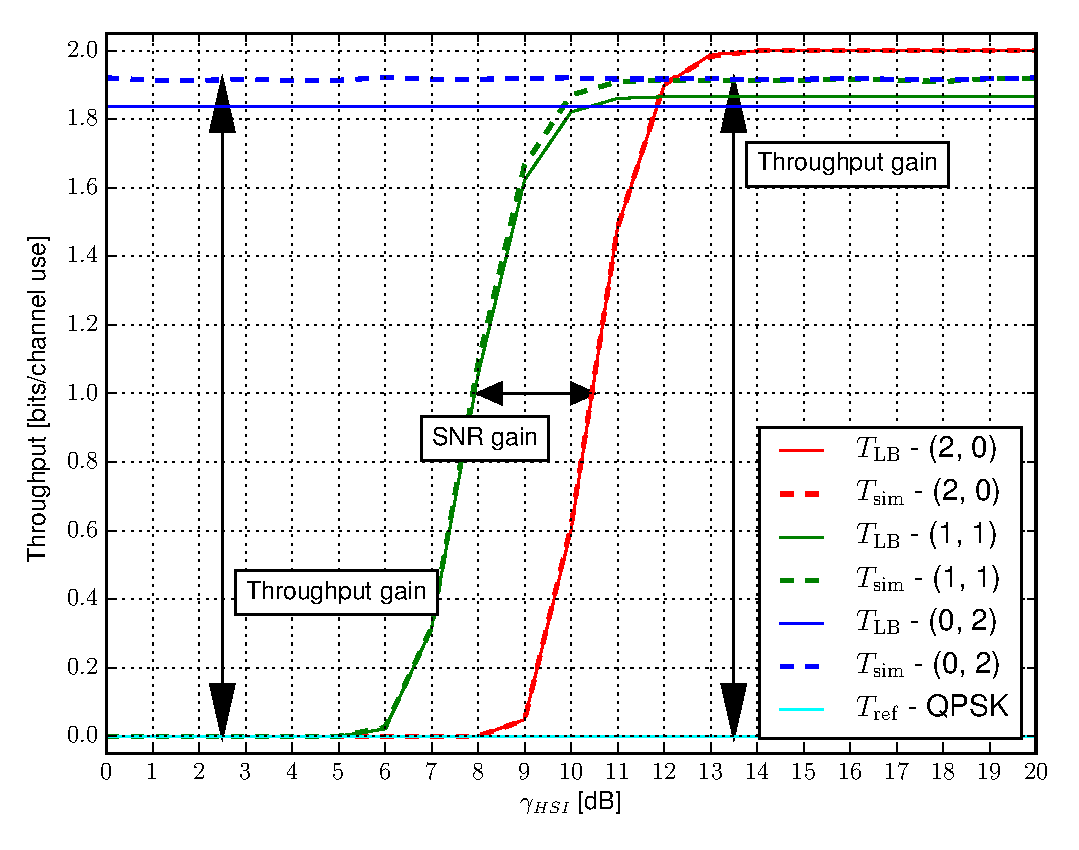
\includegraphics[width=0.45\linewidth]{fig/old_Throughput_HSI_XOR_MAC16_BC20_N2.eps}
    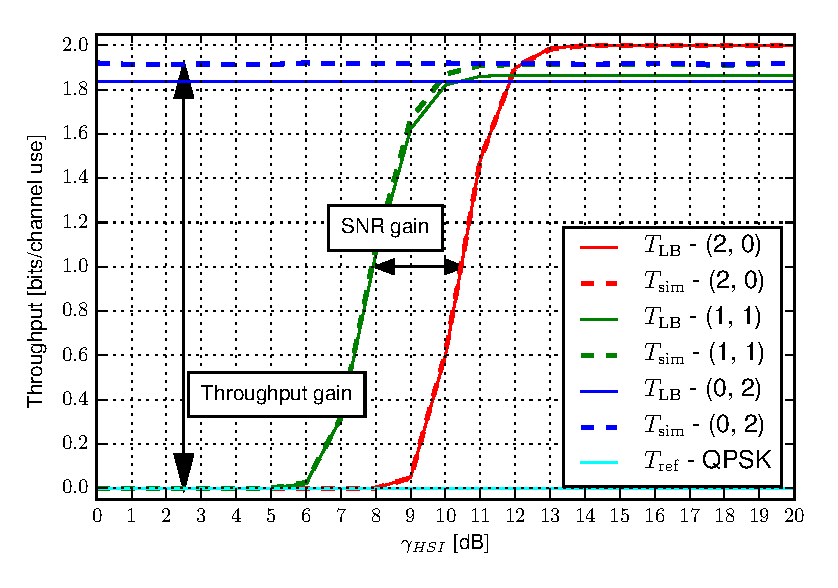
\includegraphics[width=0.45\linewidth]{fig/Throughput_HSI_XOR_MAC16_BC20_N2.eps}\\
    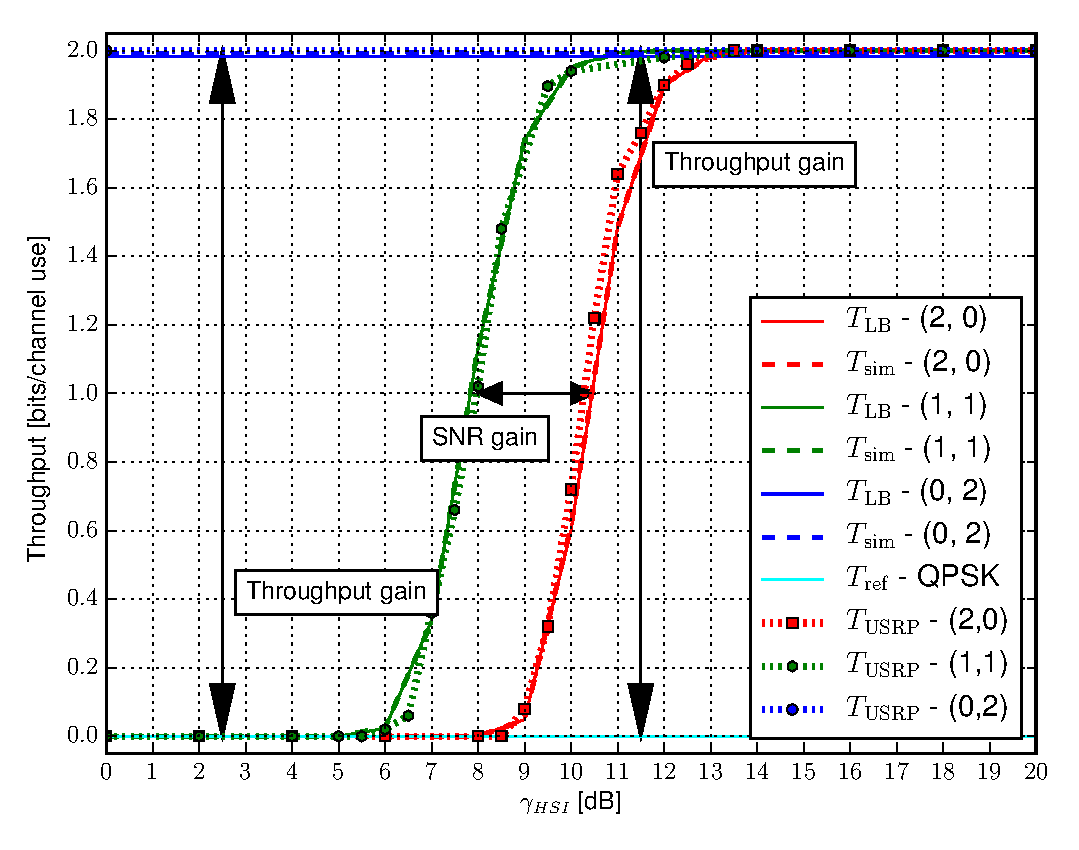
\includegraphics[width=0.45\linewidth]{fig/old_Throughput_HSI_XOR_MAC20_BC20_N2.eps}
    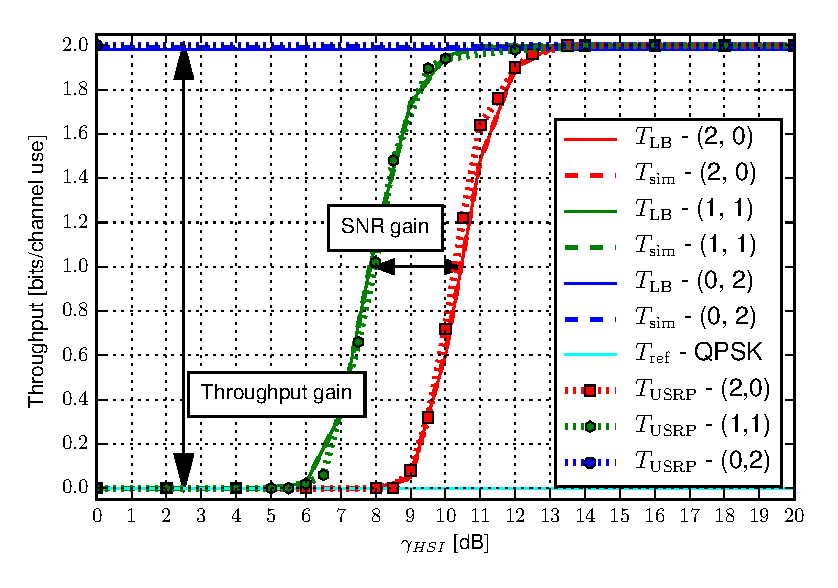
\includegraphics[width=0.45\linewidth]{fig/Throughput_HSI_XOR_MAC20_BC20_N2.eps}\\
    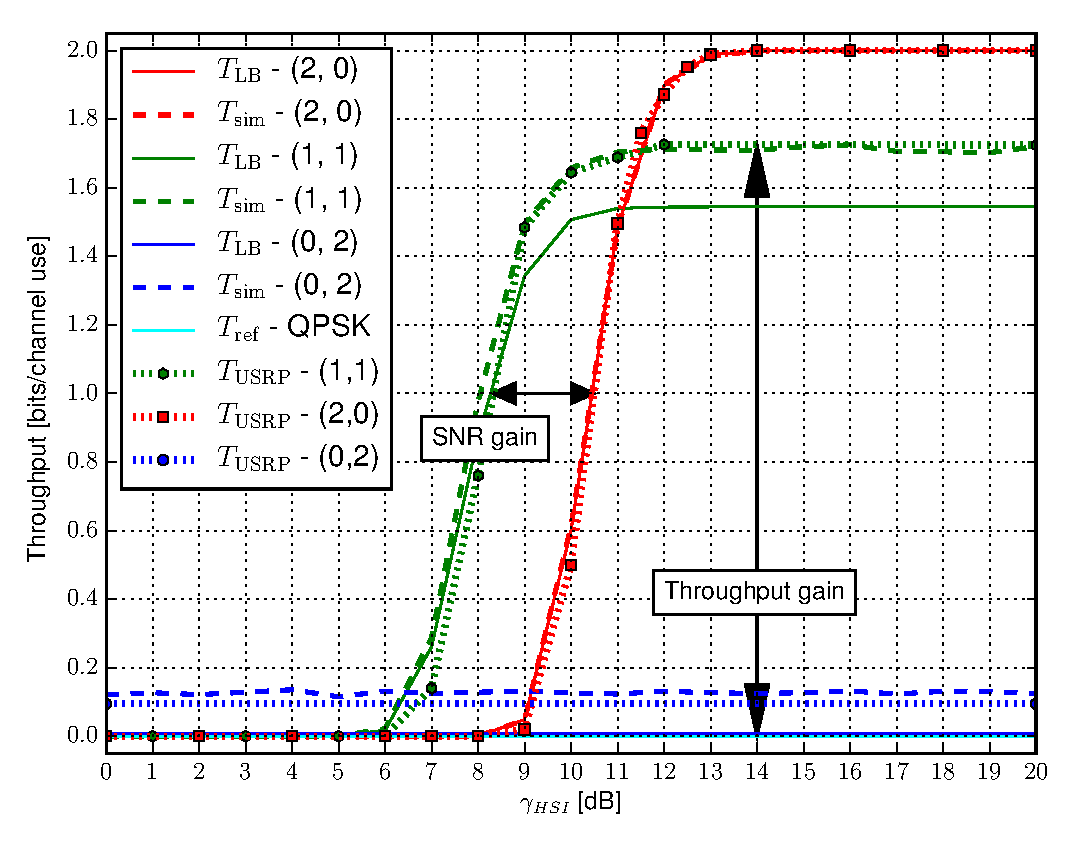
\includegraphics[width=0.45\linewidth]{fig/old_Throughput_HSI_XOR_MAC20_BC16_N2.eps}
    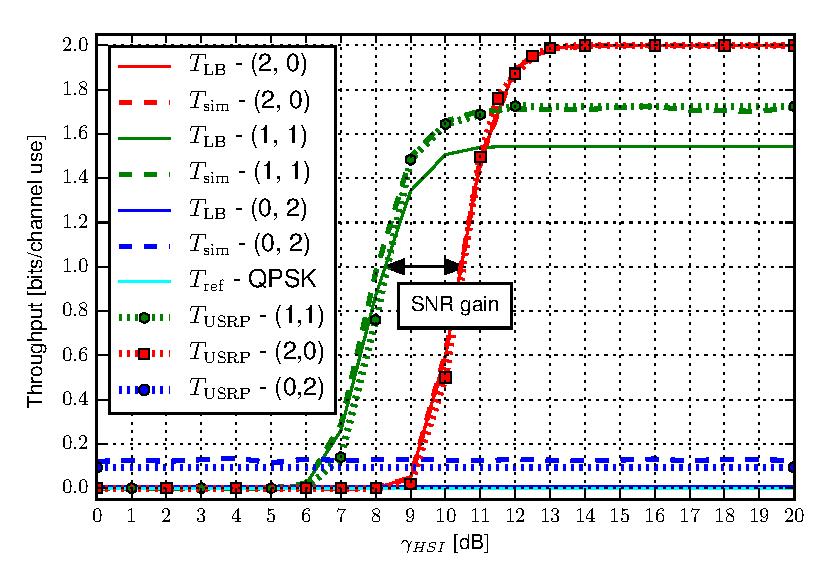
\includegraphics[width=0.45\linewidth]{fig/Throughput_HSI_XOR_MAC20_BC16_N2.eps}\\
    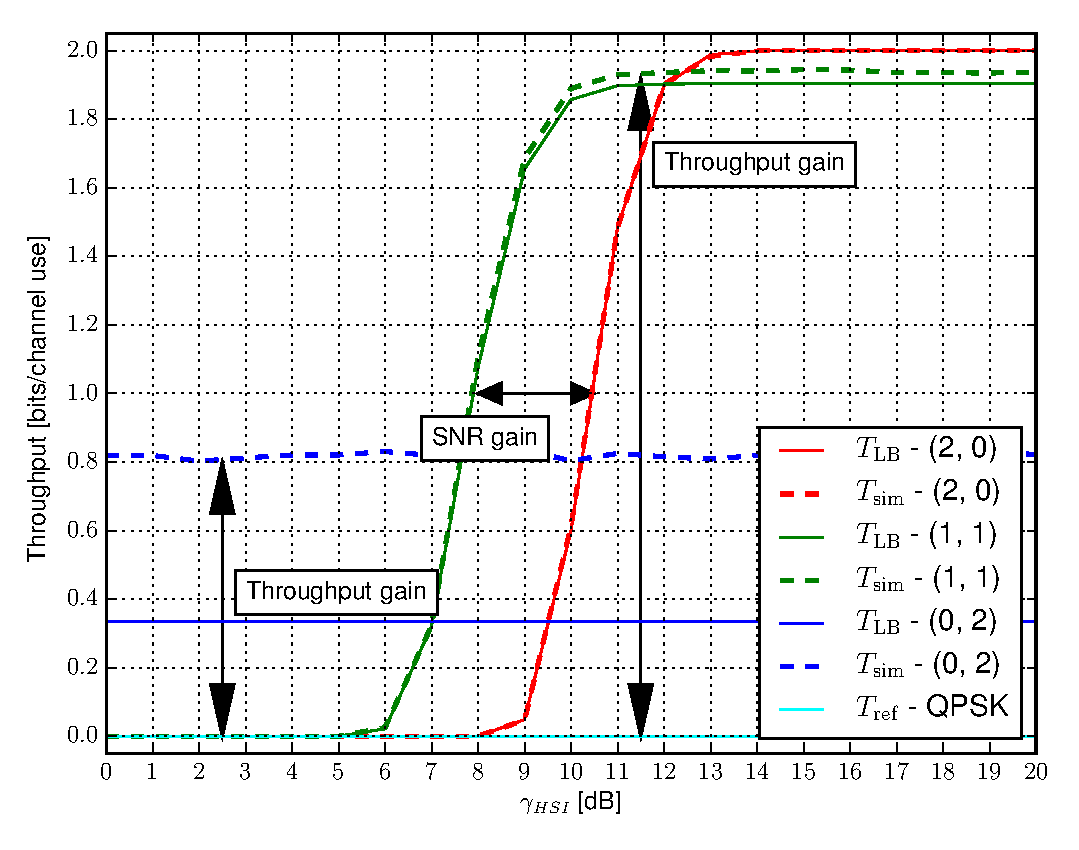
\includegraphics[width=0.45\linewidth]{fig/old_Throughput_HSI_XOR_MAC17_BC17_N2.eps}
    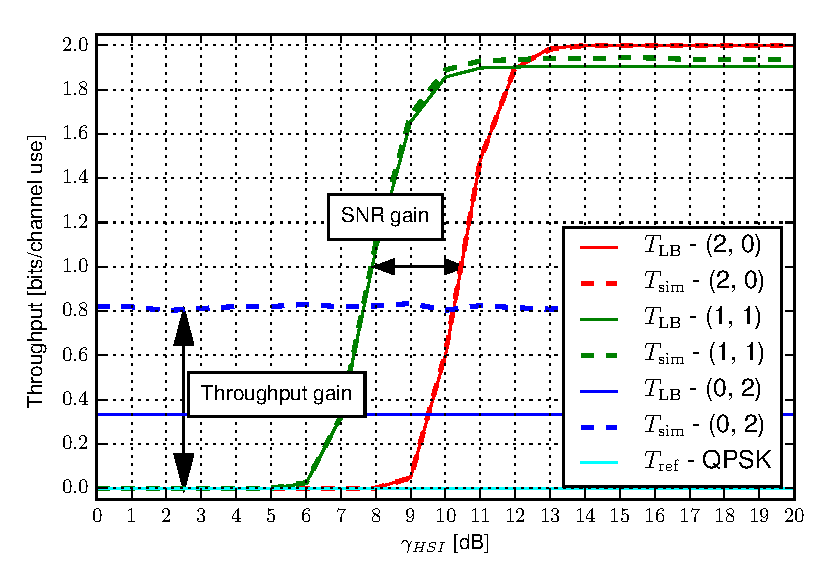
\includegraphics[width=0.45\linewidth]{fig/Throughput_HSI_XOR_MAC17_BC17_N2.eps}\\
	\caption{Uncoded throughputs (old versions left, new versions right).}
	\label{Fig:Throughput_comparison}
	%\caption{Old uncoded throughput for $\gamma_{\mathrm{MAC}}=16$,$\gamma_{\mathrm{BC}}=20$.}
    %\end{subfigure} 
    %\begin{subfigure}[t]{0.45\textwidth}
    %\caption{New the uncoded throughput for $\gamma_{\mathrm{MAC}}=16$,$\gamma_{\mathrm{BC}}=20$.}
    %\end{subfigure} 
\end{figure}

\begin{figure}
    %\begin{subfigure}[t]{0.5\textwidth}
    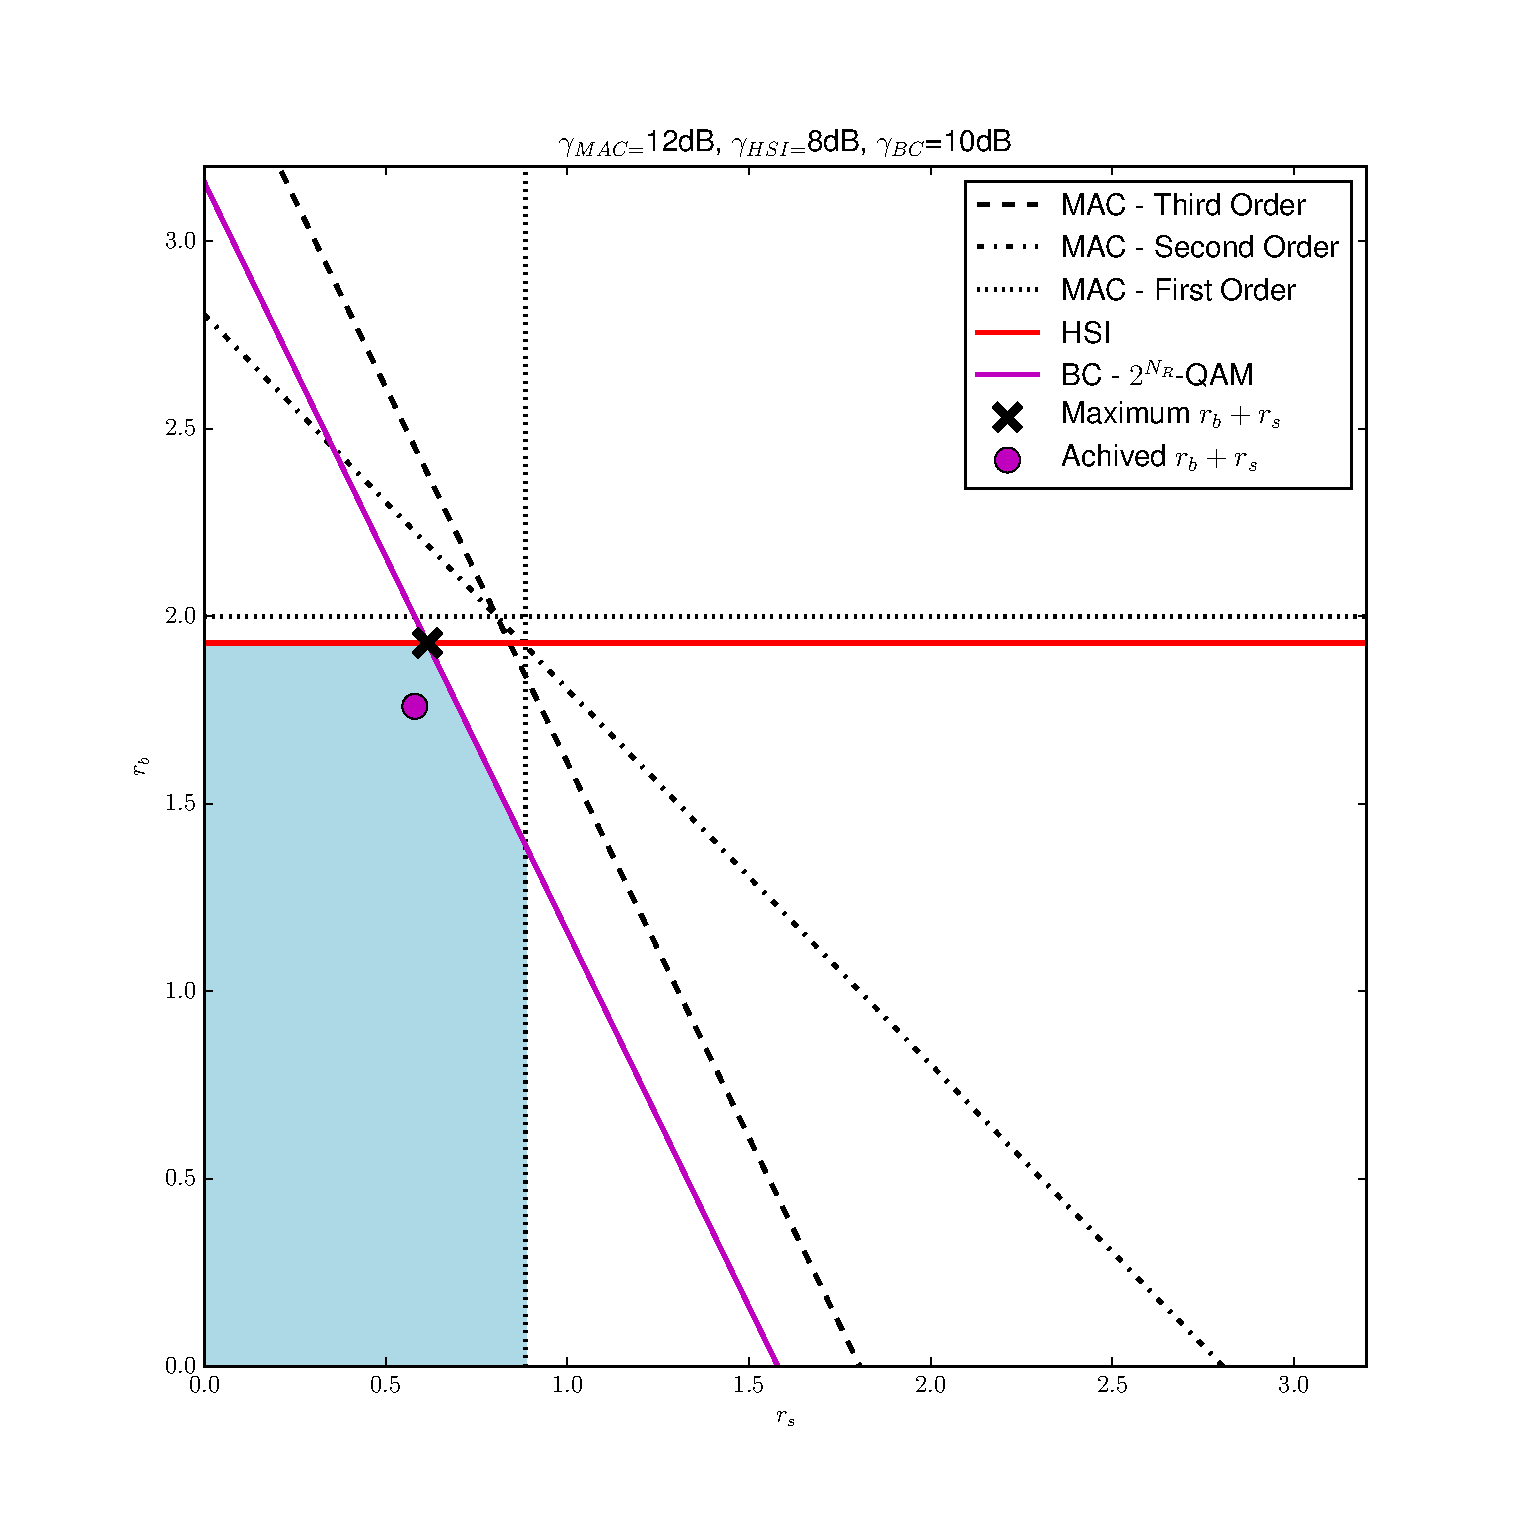
\includegraphics[width=0.45\linewidth]{fig/old_Rate_Regions_XOR_map_BC10_MAC12_HSI8.eps}
    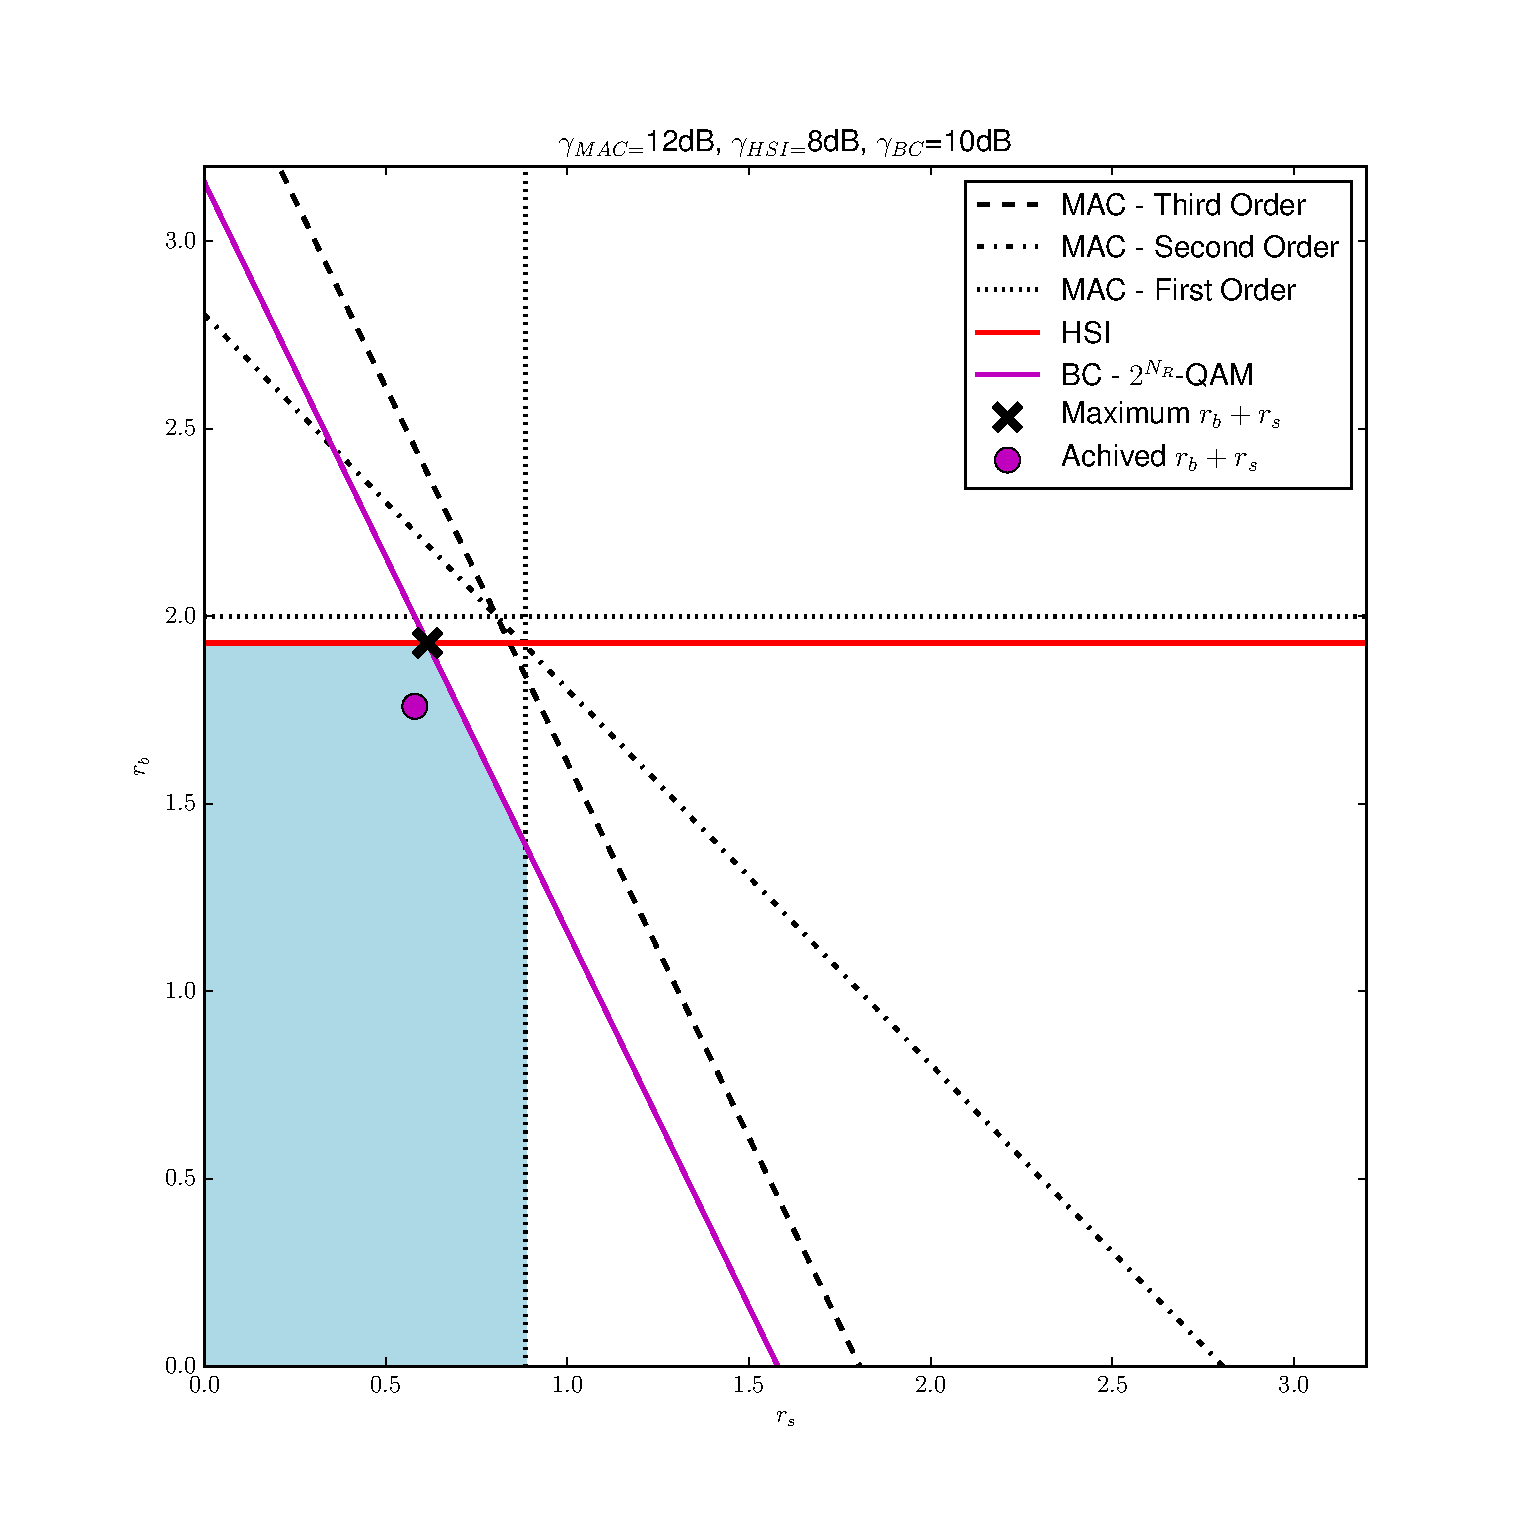
\includegraphics[width=0.45\linewidth]{../fig/Rate_Regions_XOR_map_BC10_MAC12_HSI8.eps}\\
    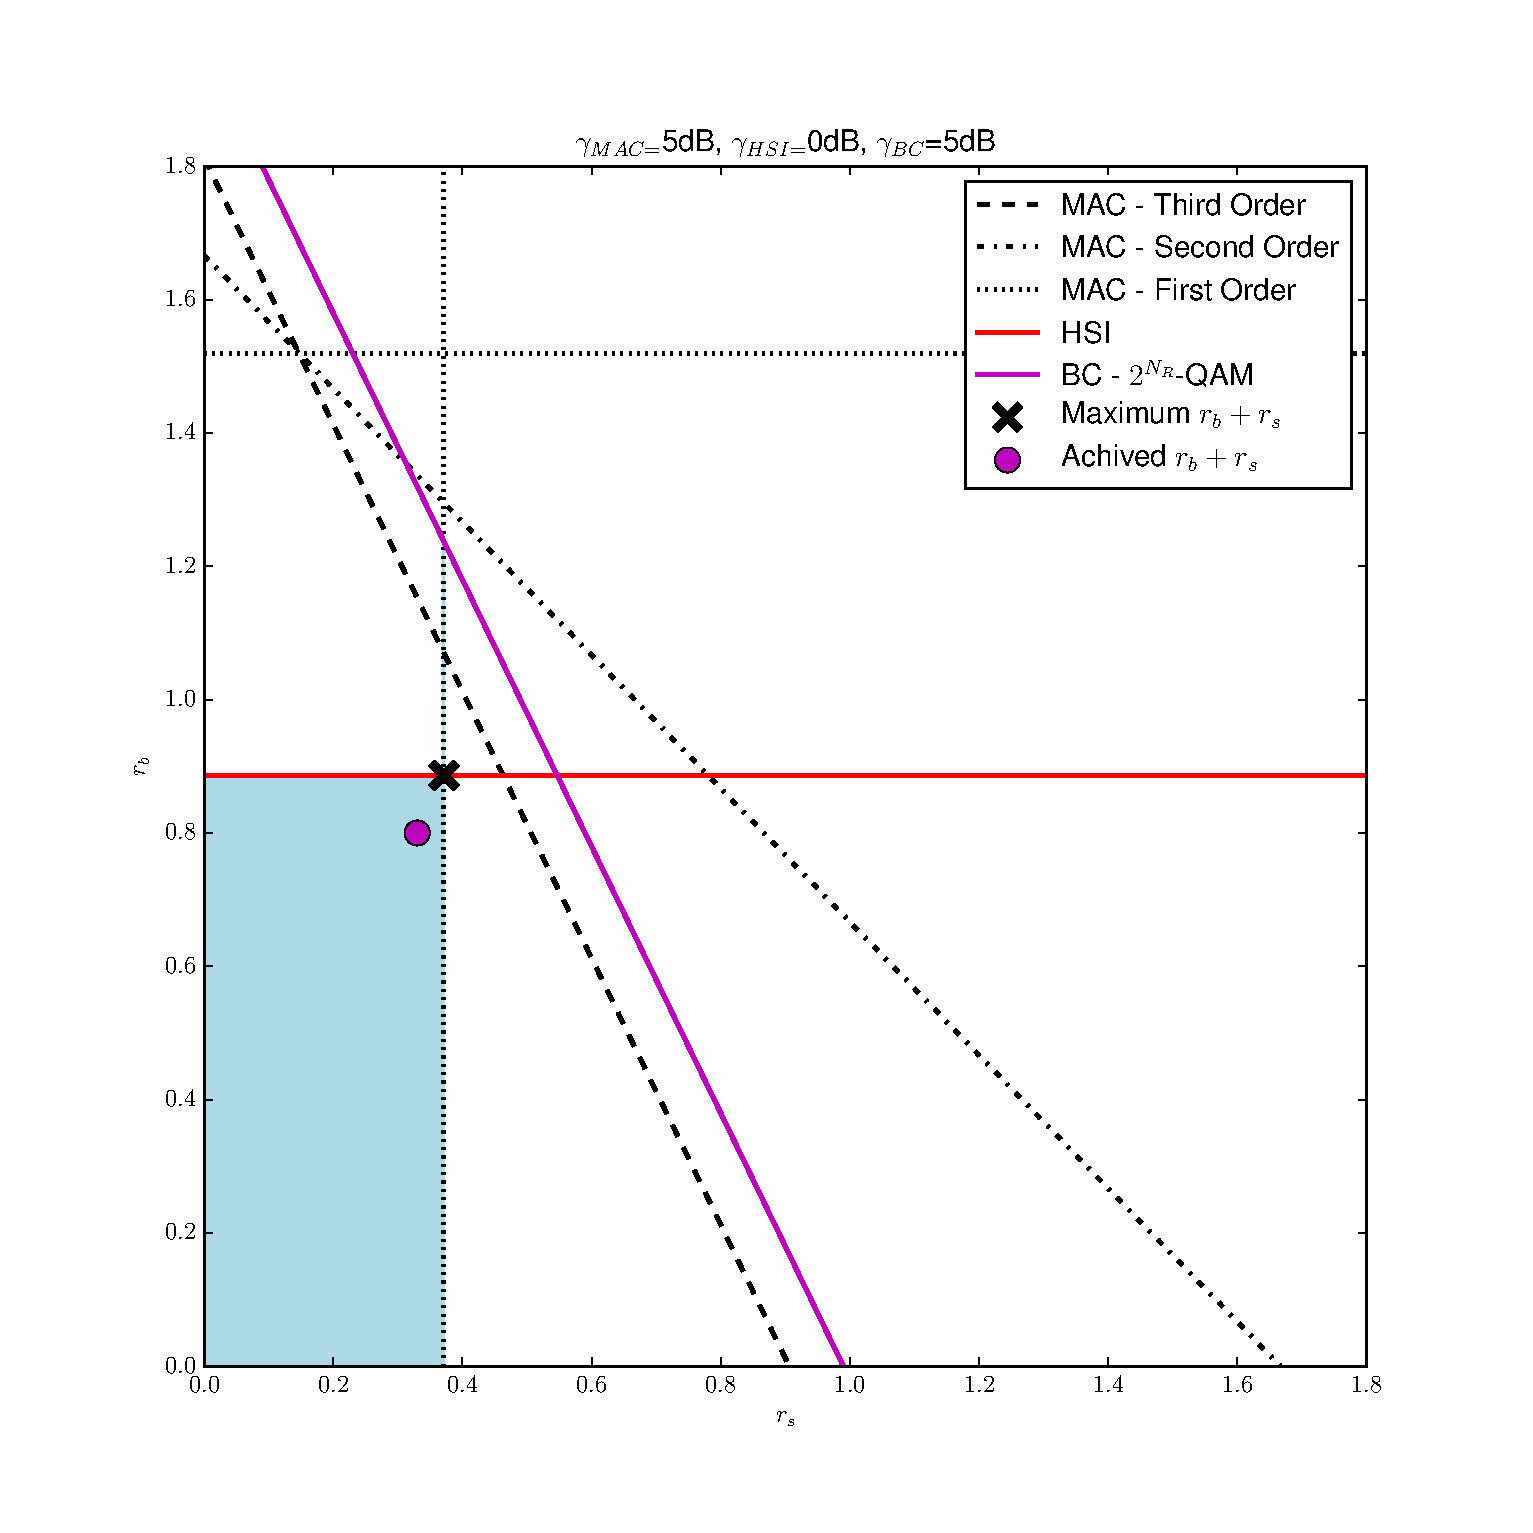
\includegraphics[width=0.45\linewidth]{fig/old_Rate_Regions_XOR_map_BC5_MAC5_HSI0.eps}
    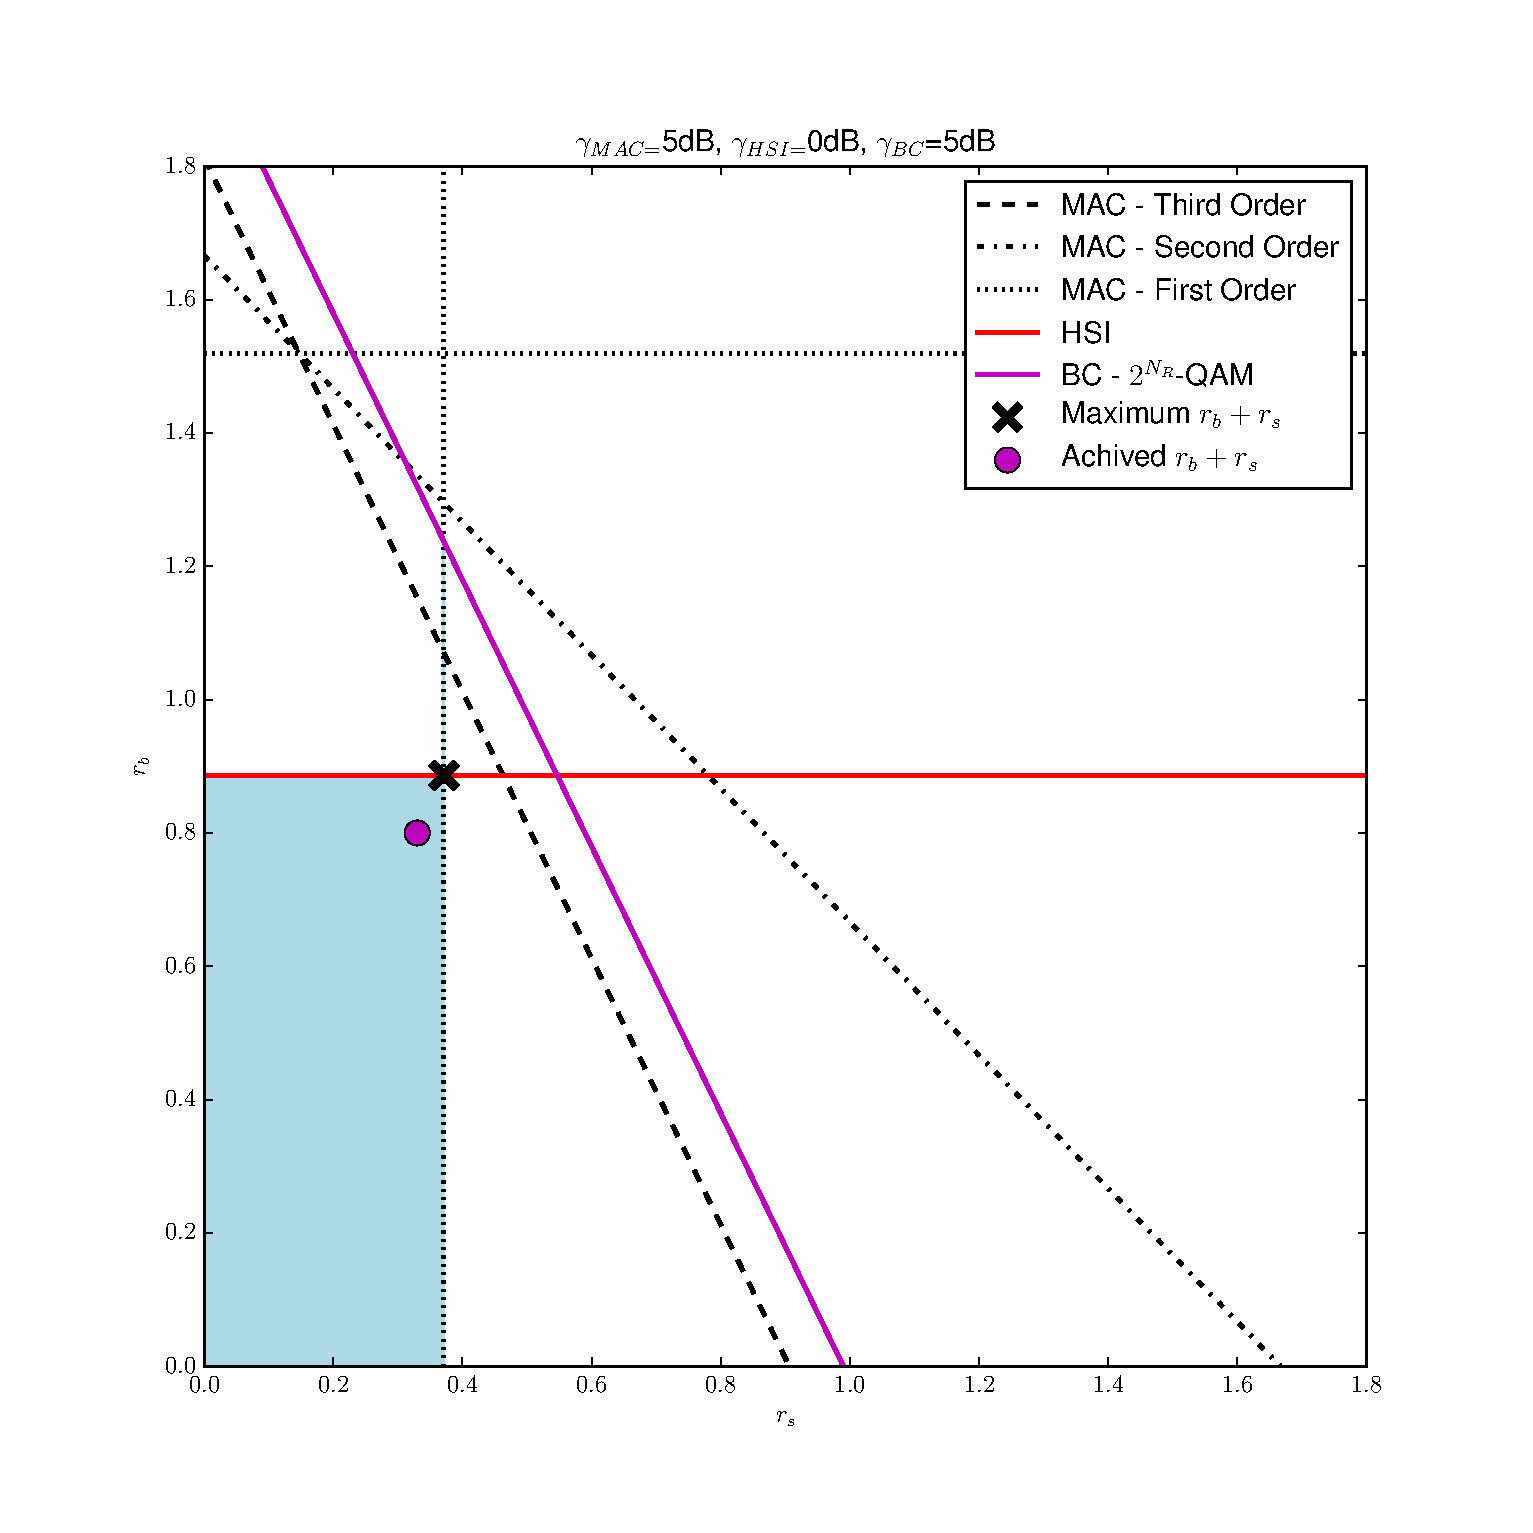
\includegraphics[width=0.45\linewidth]{../fig/Rate_Regions_XOR_map_BC5_MAC5_HSI0.eps}\\
	\caption{Enlarged fonts -- Figure 13 in the manuscript (old versions left, new versions right).}
	\label{Fig:AchievedRates}
	%\caption{Old uncoded throughput for $\gamma_{\mathrm{MAC}}=16$,$\gamma_{\mathrm{BC}}=20$.}
    %\end{subfigure} 
    %\begin{subfigure}[t]{0.45\textwidth}
    %\caption{New the uncoded throughput for $\gamma_{\mathrm{MAC}}=16$,$\gamma_{\mathrm{BC}}=20$.}
    %\end{subfigure} 
\end{figure}
\bibliographystyle{plain}
\bibliography{bib/Const_design}
\end{document}
